\section{Metodologia}\label{sec:methodology}

O estudo demonstrativo organiza o fluxo em quatro etapas: preparar os arquivos fonte, compilar o documento, executar verificações automáticas e revisar visualmente o PDF. A Figura~\ref{fig:validation-flow} resume essa sequência.

% Object example: identify the figure, declare the source, then render it.
\legend{figure}{Fluxo simplificado da validação automatizada}
\ufcSource{Elaboração própria.}
\label{fig:validation-flow}
\begin{ufcobject}[here]
  \centering
  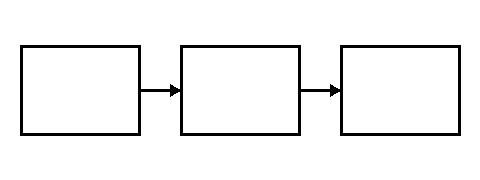
\includegraphics[width=0.65\linewidth]{figures/example-flow.png}
\end{ufcobject}

\subsection{Etapas do procedimento}

O procedimento foi organizado da seguinte forma:

\begin{enumerate}
  \item preencher os metadados e o conteúdo do documento;
  \item compilar o projeto pelo fluxo completo;
  \item verificar propriedades objetivas do PDF;
  \item inspecionar visualmente o resultado antes da entrega.
\end{enumerate}

A Tabela~\ref{tab:checks} apresenta um conjunto mínimo de verificações automáticas usado apenas como exemplo metodológico.

% Numerical table example using the tabularray module.
\begin{table}[htbp]
\centering
\begin{tallabnttblr}
[
  caption={Critérios observados no procedimento demonstrativo},
  label={tab:checks},
  remark{Fonte}={Elaboração própria.},
]
{
  colspec={X[l] X[c] X[l]},
}
\toprule
Critério & Saída & Finalidade \\
\midrule
Tamanho da página & PASS/FAIL & Confirmar o formato A4 \\
Fontes incorporadas & PASS/FAIL & Reduzir dependências externas no PDF \\
PDF/A & PASS/FAIL & Verificar o alvo arquivístico adotado \\
Marcadores estruturais & PASS/FAIL & Confirmar elementos esperados \\
\bottomrule
\end{tallabnttblr}
\end{table}

\subsection{Métrica sintética}

Para resumir uma execução didática, define-se a taxa de verificações aprovadas pela Equação~\ref{eq:pass-rate}, em que $p$ representa o número de verificações aprovadas e $n$ o total executado.

\begin{equation}
  R = \frac{p}{n}\times 100
  \label{eq:pass-rate}
\end{equation}

A métrica não representa qualidade acadêmica. Ela apenas resume o subconjunto de verificações automatizadas escolhido para o exemplo.

\subsection{Exemplo de código}

O Código~\ref{code:mean-score} mostra como incluir um arquivo externo no documento. O conteúdo é propositalmente pequeno para que o foco permaneça na estrutura do TCC.

% Code example: configure the language, identify the object and include the file.
\legend{code}{Função auxiliar para cálculo da média}
\ufcSource{Elaboração própria.}
\label{code:mean-score}
\begin{ufcobject}[here]
  \ufcInputListing[language=Python]{figures/example.py}
\end{ufcobject}

O mesmo mecanismo pode ser usado para trechos maiores, desde que o código seja relevante para o trabalho e permaneça legível no PDF.
